\section{Strategies and Justification}
A key idea that our group (and all other groups) used is to separate the strategies based on how many people are on the dance floor. However, some ideas like Hexagonal Packing are used regardless of how many dancers are present. We explain each strategy used and under what situations we used them.
\subsection{Small d - Finding all soulmates}
This is a strategy that all groups eventually converged to for small values of d. We believe that the case where d is small is “solved” in that there is no strategy better than this except for small optimizations. The key idea here is to find all dancers' soulmates. The reasoning behind this is that dancing with your soulmate gets you more points and for small values of d it's optimal to find your soulmates in the least amount of time and then dance with them. Our implementation of this is similar to group 6's implementation.\\
We start by placing the dancers in a spiral around the edges of the dance floor and leaving the centre empty. Whenever a dancer finds its soulmate, the pair leaves the dance area and goes to the centre and continues dancing there forever. \\
Note that for this idea to work, every dancer has to dance with every other dancer, otherwise there would be a possibility that some dancer would not find its soulmate and then the minimum score would be affected by this dancer which would hurt the overall score. \\
\subsubsection{The Basic Implementation}
To do this, we first place the dancers in a pairwise topology, with dancer i paired off with dancer d+1-i. Then we simply move every dancer i to the position of dancer i+1, with dancer d moving to dancer 1's location. It's easy to see that while a lot of pairs do dance together, the only pairs that dance are (i,j) where one of i and j is even and the other is odd. Most groups implemented this for their first deliverable, but our group was one of the two groups (along with group 6) that was able to fix this for our first deliverable with the change shown in the figure.\\
\subsubsection{Making All Pairs Dance}
To make even numbered dancers dance with other evens and odds with odds, we introduce a separate waiting position on the far right. On each step, instead of i going to i+1, only the dancers on the first row move one step to the right. Then we have odds and odds and evens dancing with evens. On the next step, we move the dancer on the waiting position (4 in the figure) and the dancers on the bottom row (except the dancer that is alone) to the location of dancer i+1. The dancer that is alone then moves to the location that was previously the top left corner. This introduces new dancing pairs between every turn of the previous strategy and it is easy to see that a dancer i that danced with a dancer j on one turn will on its next turn dance with dancer j-1. If j = i +1, which means that j-1 = i, on the next turn the dancer will just dance by itself. Since each dancer iterates through all the other dancers, every pair of dancers must eventually dance with each other.\\
Note that this is slightly more efficient if we use a geometry which closes the loop formed by the topology, making 4 and 8 dance with each other. In our current algorithm, on average two dancers do not dance every two turns. This means that the closed loop would only improve the score by a factor of only $\frac{1}{d}$ and we felt that we could improve our strategy in other areas instead.\\
\subsubsection{Flattening the Topology}
The difference between our and group 6's deliverable is that they flattened their topology; where two dancers were on opposite sides for our strategy, they were adjacent in group 6's. We later modified our strategy to do the same, because it made modification of the geometry easier to implement.\\
\subsubsection{The Geometry}
Our initial geometry was a circular spiral, because we thought that it would be an efficient way to pack the dancers, but we were wrong and we ended up using a rectangular spiral. The reasoning for a rectangular spiral is that pairs of dancers that have already danced have fewer movements to reach the center where they can dance forever.\\
\subsubsection{Removing Soulmate Pairs}
The final optimization we used was to make dancers who had found their soulmates leave the geometry. Our initial idea was to make all pairs dance and then pair them off. It turned out that removing them as soon as they found their soulmates was faster at pairing them and led to a higher score so we added that in.\\

\begin{figure}[h]
\center
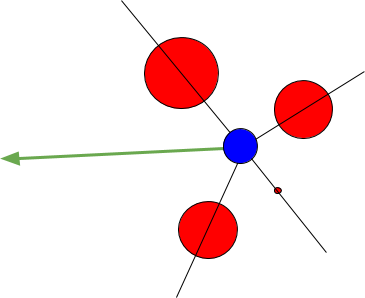
\includegraphics[scale=1]{angle.png}
\caption{}
\label{fig:angle}
\end{figure}

\\
\\


\begin{figure}[h]
\center
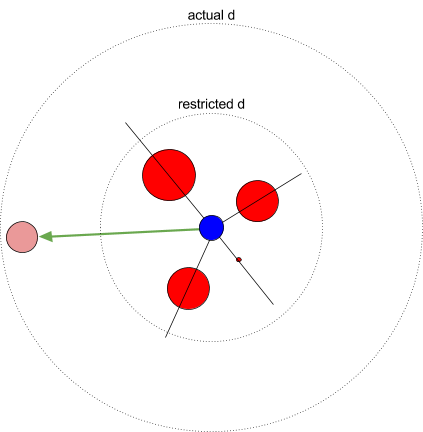
\includegraphics[scale=1]{angle2.png}
\caption{}
\label{fig:angle2}
\end{figure}

\subsection{Medium d - dance then move}
It is clear that finding all soulmates cannot work for every value of d because there is only limited time and the opportunity cost of searching for soulmates begins to outweigh the potential benefits of finding soulmates. We discuss the exact d that we chose as the upper bound for using the soulmate strategy in the parameter tuning section.\\

For much of our development process, we adopted the strategy that most groups did whereby our cells constantly moved across the board. This worked moderately well as a way to explore empty space, but we noticed that this strategy fell apart in the later stages of the game. Our blind exploration strategy was overshadowed by other groups and their clustering strategies which were able to claim more space without needing to explore all of the empty space available on the board. In the last two weeks of the project, we moved to a strategy where our cells were motionless by default. This strategy was first adopted by Group 1 as a means of naturally clustering without developing a sophisticated clustering algorithm.\\\\
We took Group 1’s basic principle and expanded upon it by creating a heuristic known as the “safe range”, which is the distance that friendly cells should ideally maintain between each other in this cluster. To make our initial cluster harder to penetrate, we wanted to limit this gap, but to make our cluster larger, we wanted to maximize this gap. This tradeoff is explained in more detail in the Parameter Tuning section where we justify the final chosen heuristic.\\\\
To execute this “safe range” heuristic, we simply employed the Largest Angle strategy discussed in the previous subsection, and set the restricted view distance to our “safe range” heuristic. By setting the restricted view distance to our “safe range” heuristic, the Largest Angle strategy in conjunction with keeping cells motionless by default naturally created a cluster of cells that were separated by no more than this “safe range”.\\\\

\subsubsection{Game State Detector}
The game has three states, the early game, the mid game, and the late game. The state is stored in memory and the transition between states depends on the number of cells near the player cell. The cell starts at the early game state, where it is motionless by default and avoids other cells by traveling toward the largest angle. The cell moves to the mid game state when there are at least three other cells within a distance of two units from it. Finally, the cell goes to the late game state when there are eight cells within a distance of two units from it. The values used to determine the state are discussed further in the parameter tuning section. The function that controls the change of state is called for each cell during each move.\\

\subsubsection{Border Strategy}
The goal of our player is to form a cluster and block off as much space as possible to grow. A key part of this is how our border cells behave in the mid game. There are a few important factors governing how our border cells behave.\\
\begin{itemize}
\item Enemy cells should not enter our cluster.
\item Our border cells should expand as the cluster grows, creating more space to grow.
\item The few stray enemy cells that enter into our cluster should be dealt with.
\end{itemize}
We divide our cells into two types: Attackers and Defenders. We decide which role they will be at the time of their creation, with attackers having a probability of $\frac{2}{3}$ and defenders having a probability of $\frac{1}{3}$. The values used here are further explained in the parameter tuning section. These values are stored in memory using one bit of information. The cells also have another parameter called the expansion ratio, which is randomly chosen from 1.0 to 2.05, in gaps of 0.15. The value (expansion ratio - 1.0)/0.15 is stored in memory, using three bits of information as this range requires numbers 0-7. These numbers are discussed in detail in the parameter tuning section.\\
A cell is determined to be on the border if:\\
\[n * (expansion ratio) > m\]
where n is the number of friendly cells and m is the number of enemy cells. A larger expansion ratio would mean that the a cell is on the border for fewer enemy cells near it, while a smaller expansion ratio will prevent the cell from expanding too fast.\\
The difference between attackers and defenders is that attackers move in a way that takes them in a direction opposite to the largest angle between enemy cells, thus moving toward enemy cells. This makes them push the borders outward, increasing the space for our cells. The problem with attackers is that they often push too far, creating gaps in the borders that allow enemy cells to enter. To solve this problem, we use defenders instead. Defenders move toward the largest angle made by friendly cells. The difference between the two is subtle, but when an enemy cell moves toward our cluster, the attackers will avoid it and keep expanding, while a defender will attempt to push it out of the cluster. If the enemy cell manages to get past the defenders however, our attackers have another purpose. On the interior of the cluster, if an attacker comes into contact with an enemy cell, it moves toward it. This causes the enemy cell to be surrounded by attackers, preventing its movement. While this might lower the number of cells that reproduce within the cluster, this does not really hurt us in the grand scheme, because eventually the cells will reproduce and fill the space anyway.
We credit group 9 for the idea of defenders, as their strategy involves making all their cells behave the same way as our defenders do. However, we found that attackers allow us to have more flexibility with expansion, which is one of the reasons we performed well in the two-player games.\\

\subsubsection{Aggressive Interior Cells}
Since we are using aggressive strategies not only restricted to the border, enemy cell inside our inner territory (which is the quite rare) actually help us a lot in packing our cell. Newly born attacker near to an enemy cell will move towards it very quickly which will later never move if no other enemy cell appear. This behavior helps us stop these cells from growing and save space later.\\
One very interesting fact we observed is that no matter in the 1-on-1 game or 9 players game, we always the last player to finish filling our space, which implies that we are the most space efficient team. This is because attacker role do not care about growing at all and often the case they are not growing. Therefore, using aggressive strategy \textbf{not only help us protect territory but also help us achieve higher packing rate.}\\

\subsubsection{Random Player}
As the game nears the late game, the best way to maximize the score is to pack cells efficiently. What our algorithm does is to try finding a direction vector using the mid game strategy. If the direction found is impossible to travel in, the cell instead looks at 10 random directions with distance sizes varying from 0.05 to 1.0 in steps of size 0.05. If it finds a direction to move that does not collide with any cell, the cell takes it.\\
We did not expect much change from adding this random fallback strategy, but surprisingly the packing greatly improved. The figure \ref{fig:random2} shows clearly how much better the random player packs cells than without it in figure \ref{fig:random1}.\\
\begin{figure}[h]
\center
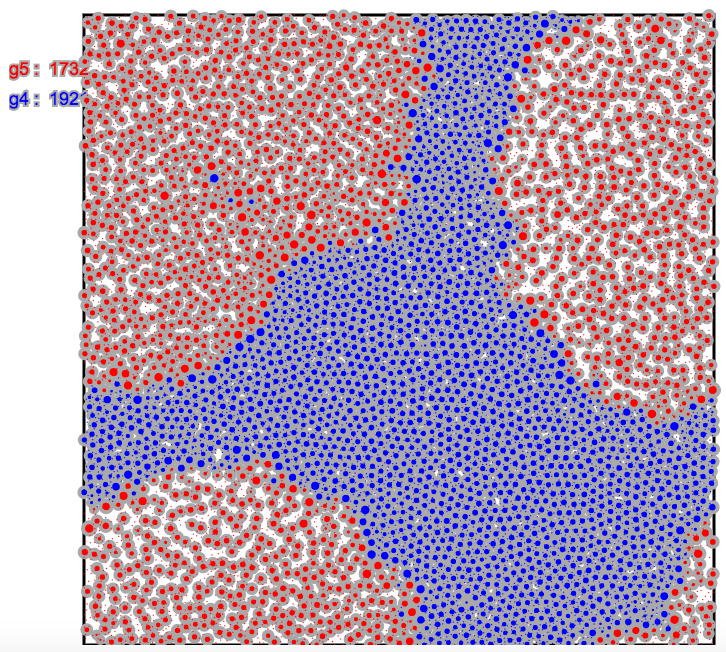
\includegraphics[scale=0.3]{random1.png}
\caption{}
\label{fig:random1}
\end{figure}

\begin{figure}[h]
\center
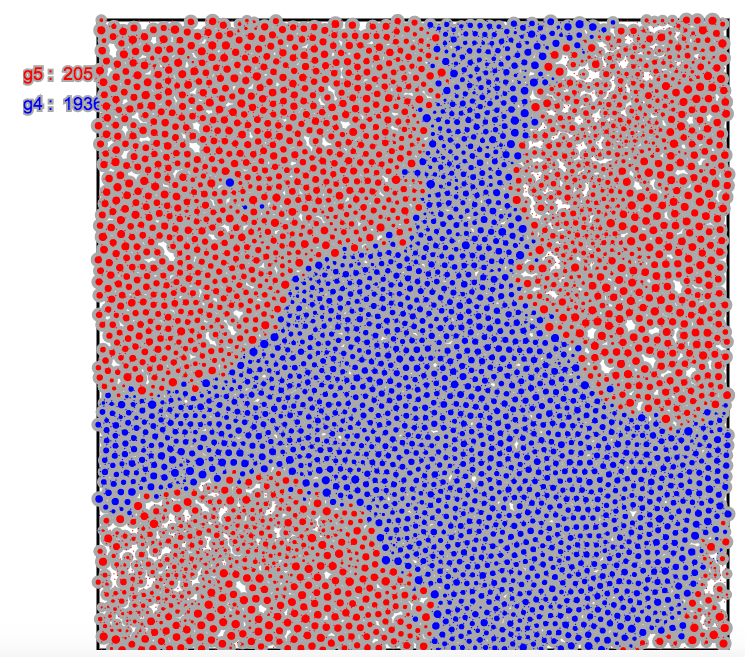
\includegraphics[scale=0.3]{random2.png}
\caption{}
\label{fig:random2}
\end{figure}

\subsubsection{Largest Traversable Distance}
We implemented a function that on input the direction would give the largest vector in the same direction that the cell could move without causing a collision. This is implemented by looking at all vectors in the direction of the input, of scale from 1.0 to 0.05, in steps of 0.05.

\subsubsection{Modified Collision Checking}
We realised that we should always allow the cell to grow after the current move is made. We modified our collision checking function to check if the cell would collide if it were 1\% larger. This gives the cell enough room to grow on its next turn.

\subsubsection{Increasing vision radius}
Our cell initially restricts its vision to a low value of 1 unit. If there are no cells within this distance, we increase the distance to 1.5 and try again. We keep repeating this until a distance of a maximum of 5 units is reached. This improved our player greatly since we were more effectively able to use larger distance values, as opposed to our earlier implementation which only looked at distances of 2 units.

\subsection{Failed Strategies}
\subsubsection{Circling Strategy}
One of the first strategies we experimented with was to form a circle of consecutive cells. The idea behind this approach was to block off a large area for our species by having cells follow each other’s pheromone trail in a circle, thus creating an impenetrable wall. We planned to have this wall expand by increasing the radius of the circle so that we would eventually have a huge area that we could later populate.\\
This strategy failed however, for two reasons. The first was that it was not obvious how to deal with reproduction of cells. Once the cell reproduced, there were two cells in its place. This would break down the pheromone circle, because two cells would compete to be in the same position in the circle.\\
The second reason this failed and consequently led us to believe that pheromone trails were not useful, is the way the cells move. The cells move from a location (x,y) to a location (x + i, y + j) by moving instantly there. What this meant was that if we tried to block space with pheromones, a cell that knew our strategy could go close to the pheromone trail and then instantly move to the other side of it. We calculated that the distance a cell had to move was only $\sqrt{r^2 - \frac{1}{2}^2}$, where r is the radius of the cell. For a cell of diameter 1, since the distance between the pheromones is 1 unit, moving between them was very easy. In fact, any cell with a diameter less than $\sqrt{2}$ could move across pheromones, breaking this strategy. The picture below shows how a cell could travel over pheromones even though the gap is smaller than its diameter.\\

\begin{figure}[h]
\center
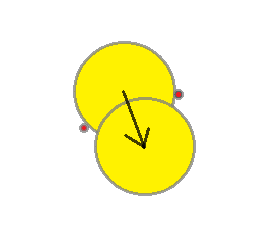
\includegraphics[scale=1]{Circle.png}
\caption{}
\label{fig:circle}
\end{figure}

\subsubsection{Purely Aggressive Strategy}
One early strategy we attempted was to be aggressive toward enemy cells when they were visible by friendly cells. The theory behind this was that we could inhibit the growth of other players by intentionally causing collisions. The inherent flaw in this strategy is that inhibiting the growth of another player will also inhibit the growth of friendly cells. The result is that this strategy works okay in pairwise competition—especially against random or naive players that don’t attempt to evade attacks, though it totally falls apart when more than two players are involved. Being aggressive against one player simply lets the third player grow unfettered. We thus learned early that having a primarily aggressive strategy. Our final strategy contained some aggressive elements as described in the Border Strategy section, but they were balanced against the competing interest of allowing friendly cells to grow.\\

\subsubsection{Tangents}
The largest angle strategy uses vectors from the center of the player cell to the center of the nearby cell. In reality, the player cell can only move along the inner tangents, as shown in the picture below.
\begin{figure}[!htb]
\center
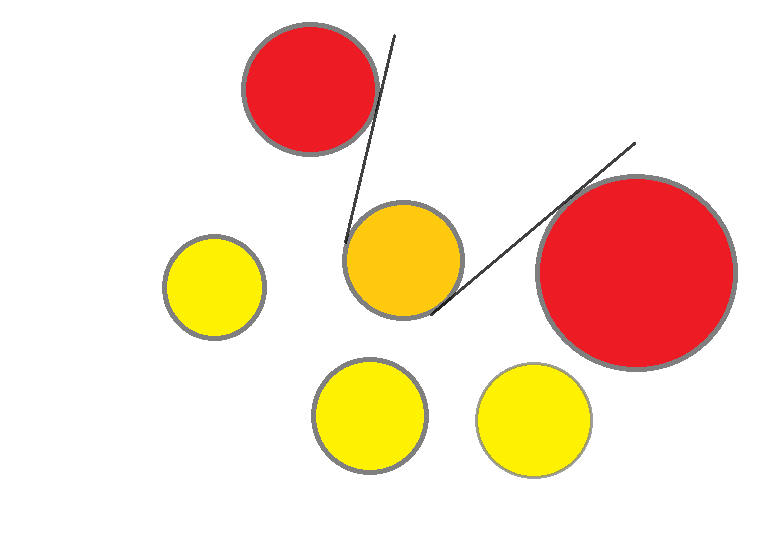
\includegraphics[scale=0.6]{tangents.png}
\caption{}
\label{fig:tangents}
\end{figure}

Our implementation for the angle strategy was changed to use the tangents instead of the centre - centre vector. We expected an improvement from this strategy.\\
However, this performed poorly and was often beaten by the simpler centre - centre vector strategy. We believe the reason for this is the implementation of movement. In the simulator, a move such as figure \ref{fig:tangents2} is considered valid.\\

\begin{figure}[!htb]
\center
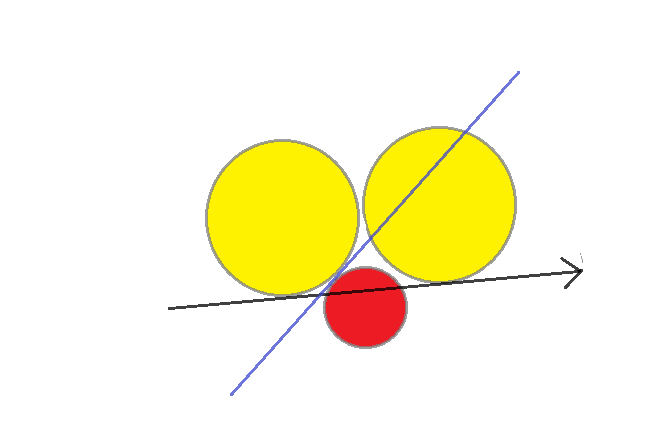
\includegraphics[scale=0.6]{tangents2.png}
\caption{}
\label{fig:tangents2}
\end{figure}

The line in blue is the tangent and the line in black, which is clearly not allowed in normal movement is still a valid move because the cell travels instantly. We abandoned this implementation because of this failure.\\

\subsubsection{Generation Tracker}
Before we used the heuristic of nearby cells to determine the current stage of the game for cell role assignment, we explored the strategy of tracking how many generations of reproduction have passed. This idea fit well with the constraints of the game since we were able to use four of the eight allowed bits in memory to keep a count of the current generation, we could increment this count on reproduction, and we could use the current generation as a heuristic to determine the role of the current cell.\\

The problem with this idea was not with the implementation, but with the fact that a generation counter is wholly insufficient when it comes detecting the current stage of the game. The number of allowable generations of reproduction within the 10mm x 10mm board depends entirely on variables unknown to the player: n, the number of starting cells for each player, and p, the total number of players on the board. In a pairwise (p=1) competition with n=1, cells could often reproduce over nine generations before a late-game strategy was viable. In a competition with p=9 and n=20, late-game conditions could appear after only three or four generations of reproduction. For this reason, we chose to abandon this strategy and use those memory bytes for the more useful purpose of maintaining a role and the randomness for expansion ratio.\\

\subsubsection{Escape Closest Cell}
Our first attempt at a late game strategy was to look at all nearby cells, pick the closest one and move in the opposite direction of it. This did not work as well as the random direction lategame strategy, so we abandoned it.\\

\subsubsection{Largest Traversable Distance using Binary Search}
The largest traversable method looks like it could use binary search in its implementaion to get more precise values than the linear check we ended up using. This turned out to not work well in practice. The reason for this is that since cells move instantly, the collision function is no longer monotonous as a function of the length of the vector.
